\documentclass[12pt]{article}
\usepackage[utf8]{inputenc}
\usepackage{csquotes}
\usepackage{hyperref}
\usepackage{authblk} % Author affiliation
\usepackage[usenames,dvipsnames]{xcolor}
\usepackage{amsfonts} % Required for mathbb
\usepackage{amsmath} % Required for alignno
\usepackage[mathlines]{lineno} % Required for line numbering
\usepackage{doi} % DOI in bibliography
% Renaming listing
\usepackage{cleveref} % Clever referencing
\Crefname{section}{Section}{Section}
% Line-numbering
\usepackage{lineno}

% For llbracket
\usepackage{stmaryrd}

\usepackage[english]{babel}
\pagenumbering{arabic}

\newenvironment{alignno}{\linenomath\align}{\endalign\linenomath}
\newenvironment{alignno*}{\linenomath\align*}{\endalign*\linenomath}

\usepackage{graphicx} % To get scale-box
% Maths commands
\usepackage{bm} % Bold maths symbols
\newcommand{\der}[2]{\frac{\partial #1}{\partial #2}}
\newcommand{\mbf}[1]{\mathbf{#1}}
\newcommand{\Int}[1]{\int\limits_{ #1}}
\newcommand{\mrm}[1]{\mathrm{#1}}
\newcommand{\mcl}[1]{\mathcal{#1}}
\newcommand{\mbb}[1]{\mathbb{#1}}
\newcommand{\mc}[2]{{\color{#1}#2}}
\newcommand{\scalemath}[2]{\scalebox{#1}{\mbox{\ensuremath{\displaystyle #2}}}}
\newcommand{\mbn}{\mbf{n}}
\newcommand{\mbu}{\mbf{u}}
\newcommand{\mbv}{\mbf{v}}
\newcommand{\mbx}{\mbf{x}}
\newcommand{\md}{\mrm{d}}
\newcommand{\norm}[1]{\left\lVert#1\right\rVert}
\newcommand{\jump}[1]{\llbracket #1 \rrbracket}
% Comment command
\setlength {\marginparwidth }{2cm}
\usepackage{todonotes}
\newcommand{\dokken}[1]{\todo[inline,color=red!50, caption={2do}]{
\begin{minipage}{\textwidth-4pt}
\underline{Dokken:} #1
\end{minipage}}}
\newcommand{\roggendorf}[1]{\todo[inline,color=green!50, caption={2do}]{
\begin{minipage}{\textwidth-4pt}
\underline{Roggendorf:} #1
\end{minipage}}}

% Bibliography imports
\usepackage[english]{babel}
\usepackage{biblatex}
\addbibresource{references.bib}

\title{Contact-conditions}
\author{J\o rgen Schartum Dokken and Sarah Roggendorf}
\affil{Department of Engineering, University of Cambridge}
\begin{document}
\maketitle
\linenumbers


%-----------------------------------Introduction-----------------------------------
In the literature one can find several methods designed for contact problems including penalty methods, Lagrange multiplier methods (LMM), augmented Lagrangian, mortar methods and Nitsche methods. Among these, mortar methods and Nitsche methods stand out due to their applicability to non-matching meshes.
It should be noted that it is somewhat misleading to list mortar methods separately from LMM since mortar methods are typically a specific realization of the Lagrange multiplier approach (though sometimes an augmented Lagrangian scheme is applied.) Both mortar and Nitsche methods have a long history in the context of finite element methods and have been widely applied in the context of domain decomposition. Even though their theoretical origins are rather different, the resulting methods are surprisingly similar. In fact, in \cite{fritz2004comparison} it is shown in the context of domain decomposition that Nitsche methods can be considered as a special case of mortar methods. In the following we will summarize the basic ideas behind these two methods and then comment on recent developments.
\section{Contact between bodies}
\subsection{Problem definition}
We start by defining our problem
\begin{subequations}
\begin{alignno}
    -\mrm{div} \sigma(\mbu)&=\mbf{f} && \text{in } \Omega,\\
    \sigma(\mbu)&=C\epsilon (\mbu)=C 0.5(\nabla \mbu + \nabla \mbu^T) && \text{in } \Omega,\\
    \mbu&=0 && \text{on } \Gamma_D\\
    \sigma (\mbu)\mbn &= \mbf{f}_N && \text{on } \Gamma_N
\end{alignno}
\end{subequations}
where $\mbn$ is the \textbf{outwards} pointing normal and $C$ is a fourth order symmetric tensor.
Note that since the stress tensor $\sigma$ is symmetric, $\mathrm{div} \sigma(\mbu)=\nabla \cdot (\sigma(\mbu)^T)=\nabla \cdot \sigma(\mbu)$,
and $\mbn\cdot \sigma(\mbu) = \sigma(\mbu)\mbn$.
To impose the Dirichlet conditions with Nitsche's method, see for instance~\cite{embar2010nitsche}.

Ignoring contributions due to contact on the contact surface $\Gamma_C$, the differential operator in its weak form is associated with the following bilinear form:

\begin{alignno}
  a(\bm u, \bm v) = \int_{\Omega} \sigma (\bm u) : \epsilon (\bm v) \md x
\end{alignno}
 and the right hand side is given by
\begin{alignno}
          l(\mbv)&=\Int{\Gamma_N}{}\mbf{f}_N\cdot \mbv\md \Gamma + \Int{\Omega}{} \mbf{f} \cdot \mbv\mrm{dx}
\end{alignno}
There is more than one way to arrive at the above linear and bilinear forms. The most natural approach in the context of Nitsche methods is to multiply the strong form of the PDE by a test function and integrate by parts. Assuming that the spaces are restricted to satisfy Dirichlet boundary conditions, the only non-zero boundary terms stemming from the integration by parts occur on the Neumann part of the boundary $\Gamma_N$ and the contact part of the boundary $\Gamma_C$. The Neumann boundary terms are included in the linear form $l$ but the terms on the contact boundary have been omitted here, since the treatment of the contact conditions is different for mortar and Nitsche methods. The same bilinear form and linear form can be derived as the first variation of the potential energy, where the contact contributions to the energy are omitted. The latter is the most natural approach in the context of mortar methods.

%----------------------------------Contact between bodies-----------------------------------------------
\subsection{Contact constraints}
In this section, we will consider two elastic bodies $\Omega_1$ and $\Omega_2$ that are expected to come in contact. Each body has a section of its boundary,
$\Gamma_{i,C}$ that might come into contact. On this surface, we define $\mbn_i$ as the outwards facing normal of the $i$th body.
Throughout this section, we will let $\Omega_1$ be the slave body, while $\Omega_2$ is the master body.
This means that we will pose all boundary conditions on the slave boundary $\Gamma_{1,D}$ as a function of the functions defined on $\Omega_2$.
\begin{figure}[!ht]
    \centering
    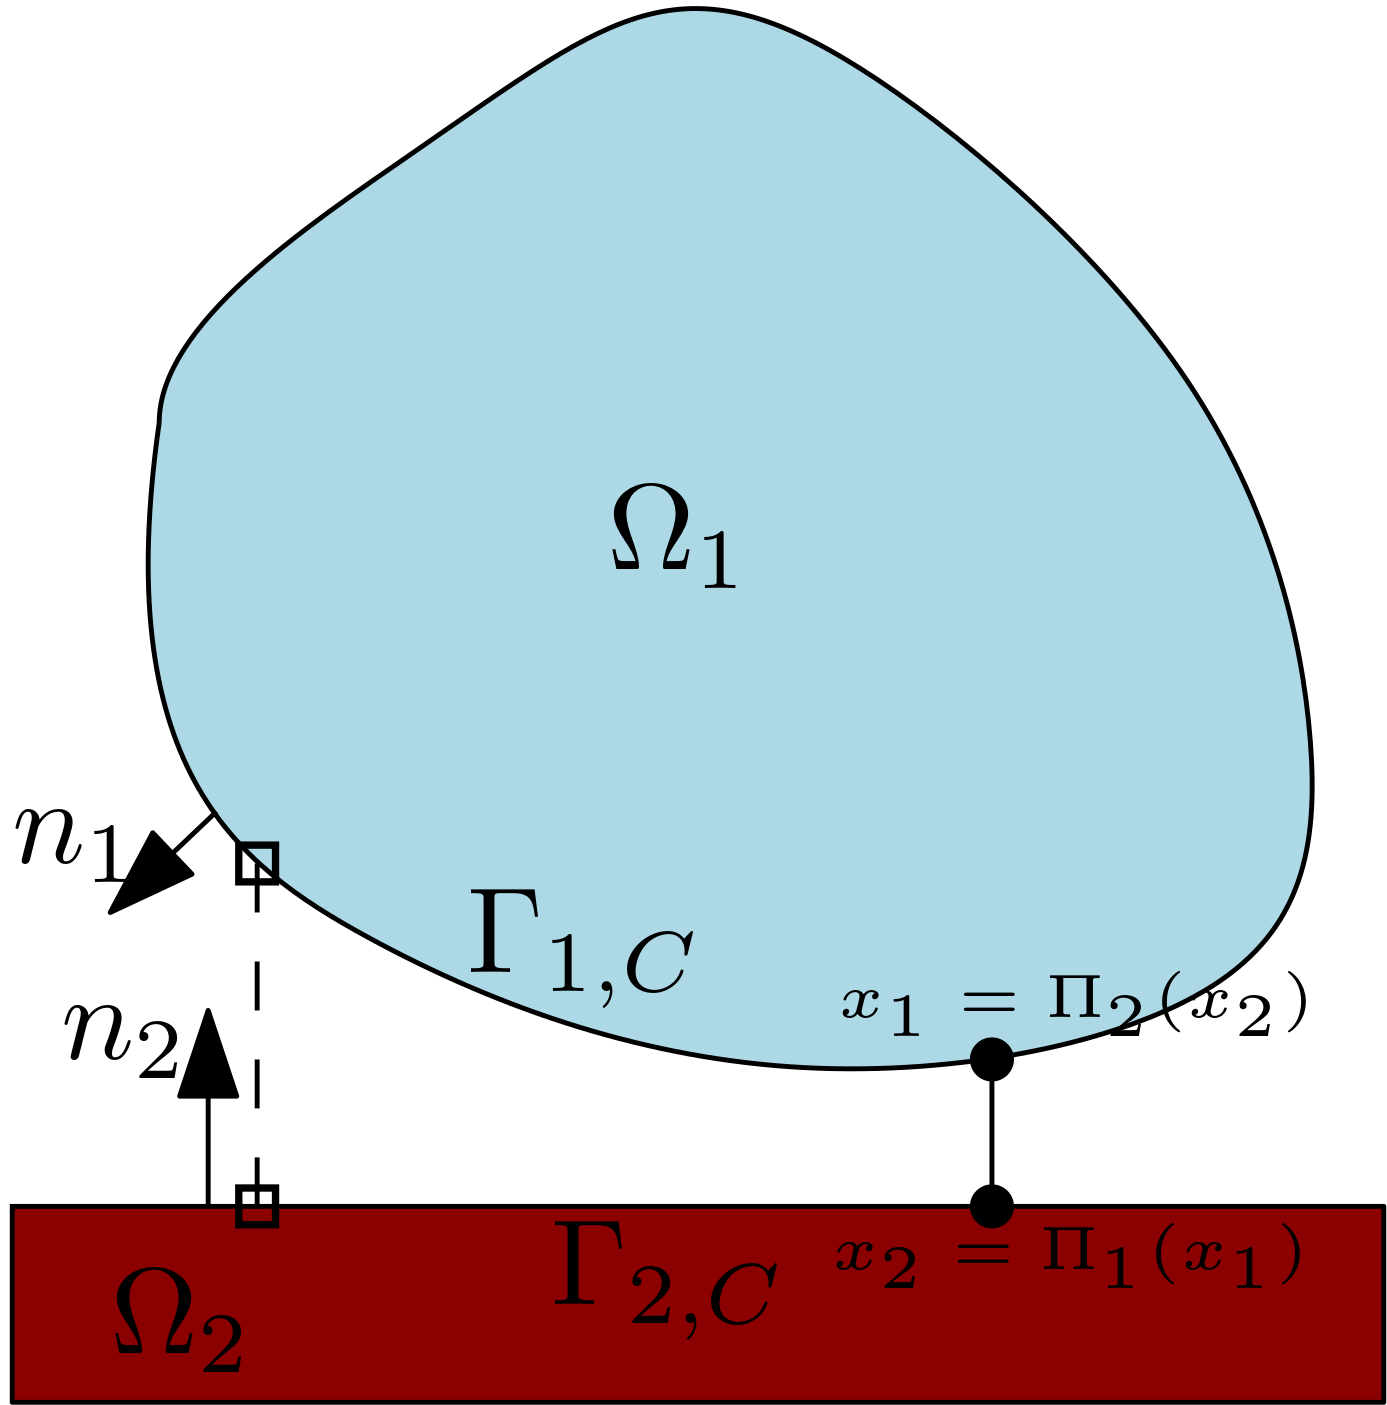
\includegraphics[width=0.5\linewidth]{contact.png}
    \caption{Illustration of two bodies and the relevant projections and normals}\label{fig:contact}
\end{figure}

We assume that the contact interfaces are sufficiently smooth, such that we can define a one to one mapping of each point of the first interface to the second interface.
We define this mapping as $\Pi_1:\Gamma_{1,C}\to \Gamma_{2,C}$. Let $J_1$ be the Jacobian of the transformation $\Pi_1$, $J_2=\frac{1}{J_1}$ the Jacobian
of $\Pi_2=(\Pi_1)^{-1}$. Further, we assume that $J_1>0$.

For any displacement field $\mbv_i$ and density surfaces forces $\sigma_i(\mbv_i)\mbv_i$ defined on $\partial\Omega_i$, we adopt the following decomposition
\begin{alignno}
    \mbv_i&= v_{i,n}\tilde{\mbn}_i+\mbv_{t,i}\\
    \sigma_i(\mbv_i)\mbn_i &= \sigma_{n,i}(\mbv_i)\tilde{\mbn}_i+\boldsymbol{\sigma}_{i,\mbf{t}}(\mbv_i)
\end{alignno}


We can write the two-body contact problem as finding the displacement field $\mbu=(\mbu_1, \mbu_2)$ subject to
\begin{subequations}
    \begin{alignno}
        \mathrm{div}\sigma_i(\mbu_i)+\mbf{f}_i&=\mbf{0} && \text{in } \Omega_i\\
        \sigma_i(\mbu_i)&= C_i\epsilon(\mbu_i) && \text{in } \Omega_i\\
        \mbu_i&=0 && \text{on } \Gamma_{i,D}\\
        \sigma_i(\mbu_i)\mbn_i&=\mbf{f}_{i,N} && \text{on } \Gamma_{i,N}
    \end{alignno}
\end{subequations}

On each surface, we define another normal $\tilde{\mbn}_i(\mbx)$ such that
\begin{alignno}
    \tilde{\mbn}_i(\mbx)&=\begin{cases}
        \frac{\Pi_i(\mbx)-\mbx}{\vert\vert \Pi_i(\mbx)- \mbx\vert\vert} &\text{if } \mbx\neq\Pi^i(\mbx)\\
        \mbf{n}_i & \text{if }\mbx=\Pi^i(\mbx)
    \end{cases}
\end{alignno}
The justification for this is that if $x=\Pi_i(x)$, there is contact between the surfaces, and the normal is simply the normal at the corresponding surface.
However, if there is a gap between the bodies, the normal vector is the normalized distance vector between the original point and its projection to the other surface.
We note that $\tilde{n}_1=-\tilde{n}_2\circ\Pi_1$ and $\tilde{n}_2=-\tilde{n}_1\circ \Pi_2$.
We define the outward unit normal $\mbn$ as the one on the master interface $\Gamma_{2,C}$:
\begin{alignno}
    \mbn = \tilde{\mbn}_2
\end{alignno}

We define the initial gap between the two bodies as done in~\cite{fabre2016SMAI}:
\begin{alignno}
    g_0:
    \begin{matrix}
        \Gamma_{1,C} \rightarrow \mathbb{R}^d\\
        \mbx \mapsto (\mbx-\Pi_1(\mbx))\cdot \mbn
    \end{matrix}
\end{alignno}
Then given a displacement field $\mbv = (\mbv_1, \mbv_2)$ defined on $\Omega_1\times\Omega_2$, the normal jump defined on the slave boundary $\Gamma_{1}$ for the normal
displacement is defined as
\begin{alignno}
    \llbracket \mbv \cdot \mbn \rrbracket(\mbx)=(\mbv_2(\Pi_1(\mbx))-\mbv_1(\mbx))\cdot \mbn(\mbx)
\end{alignno}

%-------------------Unilateral--Inequality -> equality----------------------------
\subsubsection{Unilateral contact}
We summarize the boundary conditions for unilateral contact at $\Gamma_{1,C}$:
\begin{enumerate}
    \item No penetration: $g_0-\llbracket \mbu\cdot \mbn\rrbracket \geq 0$, $\llbracket \mbu\cdot \mbn\rrbracket\leq g_0$
    \item Normal stresses on slave boundary: $\sigma_n(\mbu_1) \leq 0$
    \item Stresses only when contact: $\sigma_n(\mbu_1)(\llbracket\mbu\cdot\mbn\rrbracket-g_0)=0$
\end{enumerate}
We will use the following notation:
\begin{alignno}
   [x]_{\mathbb{R}}&=\frac{1}{2}(x-\vert x \vert)= \begin{cases}
       0 &\text{if } x\geq 0\\
       x &\text{if } x< 0
   \end{cases}
\end{alignno}
This is a projection onto $\mathbb{R}^-$.
We also define the projection onto a ball in $\mathbb{R}^d$ with radius $\alpha$ as
\begin{alignno}
   [\mbx]_\alpha &=\begin{cases}
       \mbx& \text{if } \vert \mbx \vert \leq \alpha,\\
       \alpha\frac{\mbx}{\vert\mbx\vert} & \text{otherwise}
   \end{cases}
\end{alignno}
The Heaviside function will defined such that $H(-x)+H(x)=1$, thus
\begin{alignno}
   H(x)=\begin{cases}
       1 &\text{if } x>0\\
       \frac{1}{2}& \text{if } x = 0\\
       0 &\text{if } x<0
   \end{cases}
\end{alignno}
Note that with these definitions
\begin{alignno}
   H(-x)[x]_{\mathbb{R}^-} = [x]_{\mathbb{R}^-}\label{eq:Heavi}
\end{alignno}
Using this notation, we can create an equality for the unilateral contact conditions (Similar to Proposition 2.1 in \cite{choly2013unilateral}, but using $\mathbb{R}^+$).
\begin{alignno}\label{eq:sigman:equality}
    \sigma_{n}(\mbu_1)&= \left[\sigma_n(\mbu_1) + \gamma_1(g_0- \llbracket \mbu\cdot \mbn \rrbracket)\right]_{\mathbb{R}^-}
\end{alignno}
% We prove this by considering the two cases: $\sigma_n(\mbu_1)<0$ and $\sigma_n(\mbu_1)=0$.
% We start by considering $\sigma_n(\mbu_1)<0$.
% Then the second condition imply that $\llbracket\mbu\cdot\mbn\rrbracket-g=0$, and that
% \begin{alignno}
%     \left[\sigma_n(\mbu_1) + \gamma_1(g_0- \llbracket \mbu\cdot \mbn \rrbracket)\right]_{\mathbb{R}^-}&=\left[\sigma_n(\mbu_1)\right]_{\mathbb{R}^-}=\sigma_n(\mbu_1).
% \end{alignno}
% If $\sigma_n(\mbu_1)=0$, then we have that
% \begin{alignno}
%     \left[\sigma_n(\mbu_1) + \gamma_1(g_0- \llbracket \mbu\cdot \mbn \rrbracket)\right]_{\mathbb{R}^-}&=
%     \left[\gamma_1(g_0-\llbracket\mbu\cdot\mbn\rrbracket)\right]_{\mathbb{R}^-}=0
% \end{alignno}
% as the first condition imply that $(g_0-\llbracket\mbu\cdot\mbn\rrbracket)\geq0$.

% If we assume that $\sigma_n(\mbu_1)=\left[\sigma_n(\mbu_1) + \gamma_1(g_0- \llbracket \mbu\cdot \mbn \rrbracket)\right]_{\mathbb{R}^-}$
% we have that $\sigma_n(\mbu_1)\leq 0$, fulfilling the second condition.
% We start by considering the the case when $\sigma_n(\mbu_1)=0$.
% \begin{subequations}
%     \begin{alignno}
%         \sigma_n(\mbu_1)&=\left[\sigma_n(\mbu_1) + \gamma_1(g_0- \llbracket \mbu\cdot \mbn \rrbracket)\right]_{\mathbb{R}^-}\\
%         0&=\left[0+ \gamma_1(g_0- \llbracket \mbu\cdot \mbn \rrbracket)\right]_{\mathbb{R}^-}\\
%         [g_0-\llbracket\mbu \cdot \mbn \rrbracket]_{\mathbb{R}^-}&=0\\
%         g_0-\llbracket\mbu\cdot\mbn\rrbracket&\geq0
%     \end{alignno}
% \end{subequations}
% Satisfying the first condition and the third condition, as we assumed $\sigma_n(\mbu_1)=0$.\\
%
% Next let us consider when $\sigma_n(\mbu_1)<0$. As
% \begin{align*}
%     \left[\sigma_n(\mbu_1) + \gamma_1(g_0- \llbracket \mbu\cdot \mbn \rrbracket)\right]_{\mathbb{R}^-}&=\sigma_n(\mbu_1)<0\\
%     \sigma_n(\mbu_1) + \gamma_1(g_0- \llbracket \mbu\cdot \mbn \rrbracket< 0
% \end{align*}
% This means that the $\left[\cdot\right]_{\mathbb{R}^-}$-operator is the identity mapping, and we have that
% \begin{align*}
%     \sigma_n(\mbu_1) &= \sigma_n(\mbu_1) + \gamma_1(g_0- \llbracket \mbu\cdot \mbn\rrbracket)\\
%     (g_0- \llbracket \mbu\cdot \mbn\rrbracket)&=0
% \end{align*}
% which fullfils the third condition.
%-------------------Tresca--Inequality -> equality----------------------------
\subsubsection{Tresca inequality}
For the Tresca condition,  we let $s_1\geq0$, $\llbracket\mbu\rrbracket_{\mbf{t}}=\mbu_{1,t}-\mbu_{2,t}\circ \Pi^1$ be the
relative sliding of the slave interface. The condition on the slave interface $\Gamma_{C,1}$ reads
\begin{alignno}
    &\begin{cases}
    \norm{\boldsymbol{\sigma}_{\mbf{t}}(\mbu_1)}\leq s_1& \text{if } \llbracket\mbu\rrbracket_{\mbf{t}}=0,\\
    \boldsymbol{\sigma}_{\mbf{t}}(\mbu_1)=-s_1\frac{\llbracket \mbu \rrbracket_{\mbf{t}}}{\norm{\llbracket\mbu\rrbracket_{\mbf{t}}}} & \text{otherwise}
    \end{cases}
\end{alignno}
With a similar approach as for Coulomb friction we can convert this to an equality
\begin{alignno}\label{eq:sigmat:equality}
    \boldsymbol{\sigma}_{\mbf{t}}(\mbu_1)&=\left[\boldsymbol{\sigma}_{\mbf{t}}(\mbu_1)-\gamma_1\llbracket\mbu\rrbracket_{\mbf{t}} \right]_{s_1}
\end{alignno}

%-------------------Mortar FEM---------------------------------------------------------
\section{Mortar Finite Element Methods}
This brief summary on mortar methods is mainly based on the books \cite{yastrebov2013} and  \cite{wriggers2004}.

%-------------------Method of Lagrange multipliers-------------------------------------

\subsection{Method of Lagrange multipliers (frictionless case)}
The method of Lagrange multipliers is a widely applicable approach used in optimization theory in order to find the extremum of  a functional $J(u)$ subject to contstraints of the form $g(u) = 0$, e.g.,
\begin{align*}
  \bm u^{\ast} = \mrm{arg}\min_{g(\bm u) = 0}J(\bm u).
\end{align*}
In order to transform the contstraint optimization problem into an unconstraint  problem, the so-called Lagrangian $\mcl{L}(\bm u, \lambda) = J(\bm u)+\lambda g(\bm u)$ is introduced. If now the minimum of the constraint optimization problem is attained at $\bm u^{\ast}$, there exists a $\lambda^{\ast}$ such that $\nabla \mcl{L}(\bm u^{\ast}, \lambda^{\ast}) = 0$. This is equivalent to
$\nabla J(\bm{u}^{\ast}) = -\lambda^{\ast} \nabla g(\bm u^{\ast})$ and $g(\bm{u}^{\ast}) = 0$. However, while every solution to the constraint optimization problem is a stationary point of the Lagrangian, not every stationary point is necessarily a solution to the optimization problem. Moreover, we have increased the number of degrees of freedom by introducing the Lagrange multiplier $\lambda$. Furthermore, it is important to note that if the equality constraint is replaced by an inequality constraint $g(\bm u) \leq 0$, the Lagrange multiplier approach introduces the new constraint $\lambda \leq 0$. The approach can  be extended to multiple equality and inequality constraints as well as inifinite dimensional spaces.

The starting point for the derivation of the Lagrangian for a contact formulation, is
considering the total energy $J(u) =\frac{1}{2} \int_{\Omega}\sigma(\mbu):\sigma(\mbu)-l(\mbu)$ of the two bodies in contact which is being minimized under
additional contact constraints.


We recall the frictionless contact conditions (also called Hertz-Signorini-Moreau condtions),
\begin{align*}
    g(\bm u):=  \jump{\bm u \cdot \bm n} -g_0\leq 0 \qquad \sigma_n(\mbu)\leq 0 \qquad \sigma_n(\mbu)g(\mbu) = 0 \qquad \text{on } \Gamma_C.
\end{align*}
We now aim to enforce the condition $g(\bm u) \leq 0$ on $\Gamma_C$ with the method of Lagrange multipliers. The Lagrangian in this case is given by
\begin{alignno}
  \mcl{L}(\bm u, \lambda ) = J(\bm u) + \int_{\Gamma_{1,C}} \lambda g\md \Gamma
\end{alignno}
Note that $g$ lies in a suitable trace space, and hence $\lambda$ can be identified with an element in the corresponding dual space via the Riesz representation theorem.
The gradient of $\mcl{L}$ can be determined using the notion of Gateaux derivatives which is equivalent to the first variation of the Lagrangian (also equivalent to the variational principle of virtual work). We obtain
\begin{align*}
  \nabla \mcl{L}(\bm u, \lambda)(\bm v, \mu) = a(\bm v, \bm u)-l(v)+ \int_{\Gamma_C}g \mu + \lambda_n \delta g(\bm v) \md \Gamma_C = 0 \qquad \forall (\bm v, \mu).
\end{align*}
Since the initial gap is independent of the displacement field $\mbu$, we have that $\delta g(\mbv) =  \jump{\mbv \cdot \mbn}$.
Note that we still have the additional constraint $\lambda \leq 0$, since we are enforcing an inequality constraint. If the contact surface was known exactly, the inequality constraint $g(\bm u ) \leq 0 $would be an equality constraint and we would simply have to solve a linear saddle point problem:
\begin{align*}
  a(u,v) + b(\lambda, v) &= l(v)\\
  b(\mu, u)&=0,
\end{align*}
where $b(\lambda, v)  =  \int_{\Gamma_C}\lambda \jump{\mbv \cdot \mbn} \md \Gamma$.
In particular, the resulting discretized linear problem in matrix form

\begin{align*}
  \begin{pmatrix}
    K &C\\
    C^T & 0
  \end{pmatrix}
  \begin{pmatrix}
    U\\
    \Lambda
  \end{pmatrix} =
  \begin{pmatrix}
    F\\
    0
  \end{pmatrix},
\end{align*}
where $K$ is the stiffness matrix associated with $a$ and $C$ is the discretized version of the bilinear form $b$.
It is well known, that systems of this structure must satisfy the Babuska-Brezzi (BB)-condition in order to yield a stable discretization. Whether this condition is satisfied heavily relies on the choice of discrete spaces which becomes particularly difficult if the meshes of the two bodies in contact do not align. Mortar methods are essentially characterized by a  choice of discrete spaces such that the (BB) condition is satisfied for non-matching meshes.

The other challenge that remains at this stage is that the contact surface is not known exactly and hence we have inequality constraints or in other words a non-linear problem. This so-called `active set detection' is often  realised with a semi-smooth Newton algorithm.
% \subsection{Augmented Lagrangian Approach}
% We shall not go into much detail regarding this approach. Roughly speaking, it is a combination
% of the penalty methods for enforcing contact and the LMM.
\subsection{Mortar Methods}
Mortar finite element methods were originally introduced in the context of domain decomposition.
They are combined with a  Lagrange multiplier scheme
enforcing the contact constraints. From the saddle point structure due to the use of Lagrange multipliers, mortar methods inherit the disadvantage of introducing additional degrees of freedom to the system. So-called \emph{dual} mortar approaches allow for the elimination of the additional constraints.

One aspect in which various mortar approaches differ, is the definition of the contact surface. Some
approaches introduce an intermediate surface in order to define the Lagrange multipliers on this surface, e.g., \cite{mcdevitt2000mortar}. Others choose one of the surfaces of the two bodies in contact as the mortar or master surface, e.g., \cite{wohlmuth2000mortar,krause2002dirichlet}. Combined with appropriate interpolation functions, i.e., an appropriate choice of the discrete space,  a stable method which also preserves the locality of the support of the nodal basis function can be constructed. However, this approach may not be stable when the contact occurs between curved surfaces. To remedy this so-called dual-mortar methods were designed.

The discrete space for the gap function $g(\mbu) = \jump{\mbu \cdot \mbn} -g_0$ is inherited from the discrete spaces chosen for the displacement $\mbu$.  The space for the Lagrange
multiplier $\lambda$ is yet to be chosen. In two dimensions, the basis can be chosen to be piecewise linear on the master surface except at the ends of the contacts area, where it is piecewise constant. The integration/quadrature on the slave side is more involved as a result if the meshes are not aligned. \emph{Dual} mortar methods rely on the introduction of an additional orthogonality condition on the basis of the Lagrange multiplier space, namely that the basis functions are orthogonal to the basis functions on the slave surface.
\subsection{Recent results}
\subsection{Error estimates}
One can find very little on a priori estimates for frictional contact problems. Most of the literature focuses on the frictionless case (see below). The article \cite{wohlmuth2012abstract} does include Coulomb friction in the formulation but the problem is
simplified to the frictionless case for the proof of the a priori estimates.
\begin{itemize}
  \item 2019 \cite{antolin2019priori}. Lagrange multipliers, isogeometric analysis (NURBS displacement degree $p$, Lagrange multiplier space degree $p-2$), 2D and 3D, frictionless contact. Optimal $H^1$-error $\mathcal{O}(h^{r-1})$, $r \in (1.5, 2.5)$, $\bm u \in H^r(\Omega)$ for $p \geq 2$.
  \item 2019 \cite{burman2019augmented}. Augmented Lagrangian method, Signorini/obstacle problem, 2D and 3D, existence \& uniqueness of discrete solutions. Error $\mathcal{O}(h^{r-1})$, $r \in (1.5, k+1)$, $k=1,2$ approximation order. Regularity assumption $\bm u \in H^r(\Omega)$.
  \item 2015 \cite{drouet2015optimal}. Signorini problem. 2D and 3D. Removes some of the additional assumptions in \cite{hueber2005priori} and \cite{wohlmuth2012abstract}.
   Error $\mathcal{O}(h^{\tau-1})$, $\tau \in (1.5, 1.5+k/2)$, $k=1,2$ approximation order. Regularity assumption $\bm u \in H^{\tau}(\Omega)$.
  \item 2012 \cite{wohlmuth2012abstract} Frictionless contact, abstract framework (adaptable to other Lagrange multiplier methods), 4 choices for Lagrange multiplier spaces as examples, linear and quadratic discretizations, 2D and 3D. Error $\mathcal{O}(h^{t-1})$, $t \in (2,2.5)$. Regularity assumption: $\bm u \in H^t(\Omega^{m/s})$.
  \item 2005 \cite{hueber2005priori}. Frictionless contact, primal-dual active set strategy, dual Lagrange multipliers, linear and quadratic, 2D. Error $\mathcal{O}(h^{\nu + 0.5})$, $\nu \in (0, 0.5)$, Regularity assumption: $\bm u \in H^{1.5+\nu}(\Omega^{m/s})$.
\end{itemize}

\subsection{Approximation order}
The convergence rate cannot be expected to exceed $\mathcal{O}(h^{1.5})$ due to the fact that one can not expect higher regularity of the displacement than $H^{2.5}(\Omega)$. The maximal rate can be attained by quadratic finite elements and higher order methods are therefore rarely considered. Nonetheless, it may be possible to benefit from hp-techniques, since one can expect higher regularity away from the contact surface. For an h-adaptive approach with possible p-extension see \cite{rachowicz2017h}. For large deformation with frictional sliding, the convergence rate might deterioriate and local oscillations might occur due to the low order of continuity of standard $C^0$ finite elements. In this context, it may be beneficial to apply isogeometric analysis \cite{de2011large,brivadis2015isogeometric}.

\subsection{Solution algorithm}
The inequality constraints modelling the contact of two elastic bodies introduce a non-linearity to the problem that needs to be solved with a suitable algorithm. In the context of mortar methods, one can apply a semi-smooth Newton algorithm or more specifically, a primal-dual active set strategy \cite{hintermuller2002primal} which can be combined with a multigrid preconditioner for efficiency \cite{hueber2005primal,wiesner2018algebraic}. The strategy in \cite{wiesner2018algebraic} is moreover very attractive since the additional degrees of freedom due to introduction of Lagrange multipliers are eliminated locally. The authors also consider the performance of the method in parallel.

\section{Nitsche Methods}


%------------------------ Weak formulation---------------------------------

As $\mbn$ points in the opposite direction of $\mbn_1$ where there is contact, we define the normal stresses on the slave body as
\begin{subequations}
    \begin{alignno}
        \sigma(\mbv_1)\mbn_1 &= - \sigma_n(\mbv_1)\mbn + \boldsymbol{\sigma}_{\mbf{t}}(\mbv_1),\label{eq:sigma:n1}\\
        \sigma_n(\mbv_1)&= -\sigma(\mbv_1)\mbn_1\cdot \mbn
    \end{alignno}
\end{subequations}
and similarly for the master body
\begin{subequations}
    \begin{alignno}
        \sigma(\mbv_2\circ\Pi_1(\mbx))\mbn_2(\Pi_1(\mbx))&=
        \sigma_n(\mbv_2\circ \Pi_1(\mbx))\mbn+\boldsymbol{\sigma}_{\mbf{t}}(\mbv_2\circ\Pi_1(\mbx))\label{eq:sigma:n2}\\
        \sigma_n(\mbv_2\circ \Pi_1(\mbx))&=\sigma(\mbv_2\circ \Pi_1(\mbx))\mbn_2\circ \Pi_1(\mbx)\cdot \mbn(x)
     \end{alignno}
\end{subequations}
using Newtons second law, we have that $\forall \omega\subset\Gamma_{1,C}$
\begin{alignno}
    \begin{split}
        \Int{\omega}{}\sigma (\mbu_1)\mbn\md \Gamma &= - \Int{\Pi_1(\omega)}{}\sigma(u_2)n_2\md \Gamma\\
        &= -\Int{\omega}{}\sigma(u_2\circ \Pi_1)\mbn_2 \circ \Pi_1 \vert \det(J_{\Pi_1})\vert \md \Gamma
    \end{split}
\end{alignno}
where $J_{\Pi_1}$ is the determinant of $\Pi_1$.
Therefore, we have that
\begin{alignno}\label{eq:couple:stress}
    \sigma(\mbu_1)\mbn_1 &= -\sigma(\mbu_2\circ \Pi_1)\mbn_2\circ \Pi_1 \vert \det(J_{\Pi_{1}})\vert
\end{alignno}
and have that:
\begin{alignno}
    \llbracket\sigma(\mbu)\mbn\rrbracket &= \sigma(\mbu_1)\mbn_1 + \sigma(\mbu_2\circ \Pi_1)\mbn_2\circ \Pi_1 \vert \det(J_{\Pi_{1}})\vert= 0.
\end{alignno}

We also write out this equality component-wise:
\begin{subequations}
    \begin{alignno}\label{eq:sigma_nt_cross}
        %- \sigma_n(\mbv_1)\mbn + \boldsymbol{\sigma}_{\mbf{t}}(\mbv_1) &= -\sigma_n(\mbv_2\circ \Pi_1(\mbx))\mbn\vert\det J_{\Pi_1}\vert-\boldsymbol{\sigma}_{\mbf{t}}(\mbv_2\circ\Pi_1(\mbx))\vert\det J_{\Pi_1}\vert\label{eq:sigma:n2}\\
        \sigma_n(\mbv_1)&=\sigma_n(\mbv_2\circ \Pi_1(\mbx))\vert\det J_{\Pi_1}\vert\\
        \boldsymbol{\sigma}_{\mbf{t}}(\mbv_1)&=-\boldsymbol{\sigma}_{\mbf{t}}(\mbv_2\circ\Pi_1(\mbx))\vert\det J_{\Pi_1}\vert
    \end{alignno}
\end{subequations}


As for the previous problem, we integrate by parts to find
\begin{alignno}
    \sum_{i=1,2} \Int{\Omega_i}{} \sigma(\mbu_i):\epsilon(\mbv_i)\md \Omega
    - \Int{\Gamma_{i,D}}{} \sigma(\mbu_i)\cdot \mbv_i\md \Gamma
    - \Int{\Gamma_{i,C}}{} \sigma(\mbu_i)\cdot \mbv_i\md \Gamma=L(\mbv)
\end{alignno}
where
\begin{alignno}
    L(\mbv)= \sum_{i=1,2}\Int{\Omega_i}{}\mbf{f}_i\cdot\mbv_i \md \Omega
    + \sum_{i=1,2}\Int{\Gamma_{i,N}}\mbf{l}_i\cdot \mbv_{i}\md\Gamma
\end{alignno}
We then only focus on the contact interface $\Gamma_{i,C}$, and map them to a common integration domain:
\begin{alignno}
    \begin{split}
    -\sum_{i=1,2}\Int{\Gamma_{i,C}}\sigma(\mbu_i)\mbn_i\cdot \mbv_i\md \Gamma
    =&-\Int{\Gamma_{1,C}}\sigma(\mbu_1)\mbn_1\cdot \mbv_1\md \Gamma\\
    &-\Int{\Gamma_{1,C}}\sigma(\mbu_2\circ\Pi_1)\mbn_2\circ\Pi_1\cdot \mbv_2\circ\Pi_1 \vert \det J_{\Pi_1}\vert\md \Gamma
    \end{split}
\end{alignno}
We use \cref{eq:couple:stress} such that we obtain
\begin{alignno}
    \begin{split}
    -\sum_{i=1,2}\Int{\Gamma_{i,C}}\sigma(\mbu_i)\mbn_i\cdot \mbv_i\md \Gamma
    =&\Int{\Gamma_{1,C}}-\sigma(\mbu_1)\mbn_1\cdot \mbv_1\md \Gamma
    +\sigma(\mbu_1)\mbn_1\cdot \mbv_2\circ\Pi_1 \md \Gamma\\
    =&\Int{\Gamma_{1,C}}\sigma(\mbu_1)\mbn_1\cdot(\mbv_2\circ\Pi_1-\mbv_1)\md \Gamma
    \end{split}
\end{alignno}
In turn, we use \cref{eq:sigma:n1} to rewrite our expression as
\begin{alignno}
    \Int{\Gamma_{1,C}}(-\sigma_n(\mbu_1)\mbn
    + \boldsymbol{\sigma}_{\mbf{t}}(\mbu_1))\cdot(\mbv_2\circ\Pi_1-\mbv_1)\md \Gamma\label{eq:F:body:contact}
\end{alignno}
\subsubsection{Frictionless unilateral contact}
We then have the following additional constraint:
\begin{itemize}
    \item No friction: $\boldsymbol{\sigma}_{\mbf{t}}(\mbu_1)=0$
\end{itemize}

We use this condition \cref{eq:F:body:contact} to obtain:
\begin{alignno}
    -\sum_{i=1,2}\Int{\Gamma_{i,C}}\sigma(\mbu_i)\mbn_i\cdot \mbv_i\md \Gamma
    =&-\Int{\Gamma_{1,C}}\sigma_n(\mbu_1)\cdot \llbracket \mbv\cdot \mbn\rrbracket\md \Gamma
\end{alignno}
and therefore we have that
\begin{alignno}
    a(\mbu,\mbv)&= \sum_{i=1,2} \Int{\Omega_i}{} \sigma(\mbu_i):\epsilon(\mbv_i)\md \Omega
    - \Int{\Gamma_{i,D}}{} \sigma(\mbu_i)\cdot \mbv_i\md \Gamma
    -\Int{\Gamma_{1,C}}\sigma_n(\mbu_1)\cdot \llbracket \mbv\cdot \mbn\rrbracket\md \Gamma
\end{alignno}
\subsubsection{Tresca friction}
Starting from \cref{eq:F:body:contact} we have
\begin{alignno}
    \begin{split}
        - \Int{\Gamma_{i,C}}{} \sigma(\mbu_i)\cdot \mbv_i\md \Gamma&= \Int{\Gamma_{1,C}}(-\sigma_n(\mbu_1)\mbn
        + \boldsymbol{\sigma}_{\mbf{t}}(\mbu_1))\cdot(\mbv_2\circ\Pi_1-\mbv_1)\md \Gamma\\
        &= -\Int{\Gamma_{1,C}}\sigma_n(\mbu_1) \llbracket \mbv\cdot \mbn\rrbracket\md \Gamma
        -\Int{\Gamma_{1,C}}\boldsymbol{\sigma}_{\mbf{t}}(\mbu_1)\cdot \llbracket \mbv\rrbracket_\mbf{t}\md \Gamma
    \end{split}\label{eq:tresca:1}
\end{alignno}

We modify this by using:
\begin{subequations}
    \begin{alignno}
        \llbracket\mbv \cdot \mbn \rrbracket&=
        -\frac{1}{\gamma_1} (\theta\sigma_n(\mbv_1)
        -\gamma_1 \llbracket\mbv\cdot\mbn\rrbracket)
        + \frac{\theta}{\gamma_1}\sigma_n(\mbv_1)\\
        \llbracket\mbv\rrbracket_{\mbf{t}}&=
        -\frac{1}{\gamma_1} (\theta\boldsymbol{\sigma}_\mbf{t}(\mbv_1)
        -\gamma_1 \llbracket\mbv\rrbracket_\mbf{t} )
        + \frac{\theta}{\gamma_1}\boldsymbol{\sigma}_\mbf{t}(\mbv_1)
\end{alignno}
\end{subequations}
For the normal component we get
\begin{alignno}
    \begin{split}
    -\Int{\Gamma_{1,C}}\sigma_n(\mbu_1) \llbracket \mbv\cdot \mbn\rrbracket\md \Gamma &=
    \Int{\Gamma_{1,C}}\sigma_n(\mbu_1) \frac{1}{\gamma_1} (\theta\sigma_n(\mbv_1)
    -\gamma_1 \llbracket\mbv\cdot\mbn\rrbracket)
    -\sigma_n(\mbu_1)\frac{\theta}{\gamma_1}\sigma_n(\mbv_1)\md \Gamma\\
    &=-\Int{\Gamma_{1,C}}{}\frac{\theta}{\gamma_1}\sigma_n(\mbu_1)\sigma_n(\mbv_1)\md \Gamma\\
    &+\Int{\Gamma_{1,C}}{}\frac{1}{\gamma_1}\left[\sigma_n(\mbu_1)
    +\gamma_1(g-\llbracket\mbu\cdot\mbn\rrbracket \right]_{\mathbb{R}^-})(\theta\sigma_n(\mbv_1)
    -\gamma_1 \llbracket\mbv\cdot\mbn\rrbracket)\md \Gamma
    \end{split}
\end{alignno}
where the latter equality comes from applying \cref{eq:sigman:equality}
Similarly for the tangential component, we obtain:
\begin{alignno}
\begin{split}
    -\Int{\Gamma_{1,C}}\boldsymbol{\sigma}_{\mbf{t}}(\mbu_1)\cdot \llbracket \mbv\rrbracket_\mbf{t}\md \Gamma
    &=\Int{\Gamma_{1,C}}\frac{1}{\gamma_1} \boldsymbol{\sigma}_{\mbf{t}}(\mbu_1)\cdot
    (\theta\boldsymbol{\sigma}_\mbf{t}(\mbv_1) -\gamma_1 \llbracket\mbv\rrbracket_\mbf{t} )\md \Gamma\\
        &-\Int{\Gamma_{1,C}} \frac{\theta}{\gamma_1}\boldsymbol{\sigma}_{\mbf{t}}(\mbu_1)\cdot\boldsymbol{\sigma}_\mbf{t}(\mbv_1)
\md \Gamma\\
&=-\Int{\Gamma_{1,C}} \frac{\theta}{\gamma_1}\boldsymbol{\sigma}_{\mbf{t}}(\mbu_1)\cdot\boldsymbol{\sigma}_\mbf{t}(\mbv_1)\md \Gamma\\
 &+\Int{\Gamma_{1,C}}\frac{1}{\gamma_1}\left[\boldsymbol{\sigma}_{\mbf{t}}(\mbu_1)-\gamma_1\llbracket\mbu\rrbracket_{\mbf{t}} \right]_{s_1}\cdot
(\theta\boldsymbol{\sigma}_\mbf{t}(\mbv_1) -\gamma_1 \llbracket\mbv\rrbracket_\mbf{t} ) \md \Gamma
\end{split}
\end{alignno}
Summarizing, we have that
\begin{alignno}
    \begin{split}
    - \Int{\Gamma_{i,C}}{} \sigma(\mbu_i)\cdot \mbv_i\md \Gamma&=
    -\Int{\Gamma_{1,C}}{}\frac{\theta}{\gamma_1}\left(\sigma_n(\mbu_1)\sigma_n(\mbv_1)+\boldsymbol{\sigma}_{\mbf{t}}(\mbu_1)\cdot\boldsymbol{\sigma}_\mbf{t}(\mbv_1)\right)\md \Gamma\\
    &+\Int{\Gamma_{1,C}}{}\frac{1}{\gamma_1}\left[\sigma_n(\mbu_1)
    +\gamma_1(g-\llbracket\mbu\cdot\mbn\rrbracket \right]_{\mathbb{R}^-})(\theta\sigma_n(\mbv_1)
    -\gamma_1 \llbracket\mbv\cdot\mbn\rrbracket)\md \Gamma\\
 &+\Int{\Gamma_{1,C}}\frac{1}{\gamma_1}\left[\boldsymbol{\sigma}_{\mbf{t}}(\mbu_1)-\gamma_1\llbracket\mbu\rrbracket_{\mbf{t}} \right]_{s_1}\cdot
(\theta\boldsymbol{\sigma}_\mbf{t}(\mbv_1) -\gamma_1 \llbracket\mbv\rrbracket_\mbf{t} ) \md \Gamma
    \end{split}
\end{alignno}

%------------------------ Weak formulation---------------------------------
\subsection{Recent results}
\begin{itemize}
\item 2004: Nitsche method for elasticity problems with strong discontinuity originated in~\cite{HANSBO20043523} (2D/3D). 
Here elements with internal discontinuities were enriched by "duplicating" the element, having it as part of both sides of the cell/facet integrals.
For first order linear elements, second order convergence in ($L^2$) is proven. Also considers numerical study of frictionless contact (and crack propagation), with a fixed point iteration scheme
\item 2013: Convergence proofs extended to the $H^1(\Omega)$ norm in~\cite{choly2013unilateral} (2D), of order $H^{\frac{1}{2}+\nu}$ provided solution regularity of $H^{\frac{3}{2}+\nu}$, $\nu\in(0,\frac{1}{2}]$.
Linear and quadratic elements considered.
Shows that their approach can be viewed as a mixed (Lagrange multiplier method) with an additional stabilization term (and a different Lagrange multiplier space).
\item 2015: Two new methods for apply Nitsche's method to unilateral contact is presented in~\cite{chouly2015symm}. 
One non-symmetric and one skew-symmetric method, where the latter is quite similar to a penalty approach (2D/3D). Proves similar convergence estimates as~\cite{choly2013unilateral}.
Skew symmetric case preserves optimal convergence irrespective of the value of the Nitsche parameter.
\item  2013: Nitsche's method with Coulomb friction is presented and a numerical study is performed~\cite{RENARD201338}. 
Minimal Nitsche parameter for coercivity estimated by the smallest eigenvalue of tangent matrix. Unsymmetric version shows improved convergence and requires a smaller Nitsche parameter.
\item 2013: Nitsche's method with Tresca friction~\cite{CHOULY2014TRESCA}. Same $\theta$ strategy as~\cite{chouly2015symm} and optimal convergence results as ~\cite{choly2013unilateral} (2D/3D, piecewise linear and quadratic elements). Claims results can be extended to bilateral contact with Tresca friction.
\item 2015: Time-marching schemes for unilateral contact with Nitsche's method is introduced in~\cite{chouly2015timedep} ($\theta$ and hybrid schemes). Proves well-posed and conservation of augumented energy. Numerical study and stability estimates in ~\cite{chouly2015timedep2}.
\item 2017: ~\cite{MLIKA2017selfcontact}
\end{itemize}
%-------------------Mortar finite element formulations---------------------------------



%-------------------Bibliography-----------------------
\printbibliography

\end{document}
